It is possible to come up with several paradoxes by using a vague notion of limit. For example, the following proof called the Staircase Paradox {\it ``proves''} that $4 = \pi$.
\begin{exercise}
	What (if anything) is wrong with the following proof? \footnote{This is just a fun problem. It's ok to be vague in your answer.}
	\begin{claim} $4 = \pi$.
	\end{claim}
	\begin{proof}
		\begin{figure}[H]
			\centering
			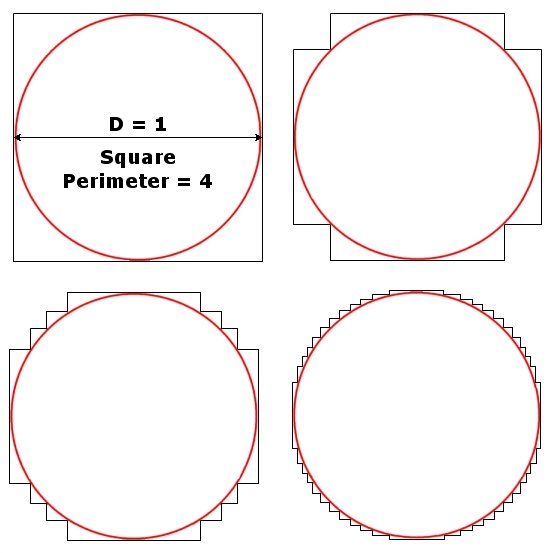
\includegraphics[width=0.6\textwidth]{pi4.jpg}
		\end{figure}
		\begin{enumerate}
			\item
			      Start with a circle inscribed inside a square.
			\item
			      `Invert' the corner of the square so that the resulting polygon, which has the same perimeter (= 4) as the square, better approximates the circle.
			\item Repeat the process.
			\item In the limit we approach the circle hence $\pi = 4$.
		\end{enumerate}
	\end{proof}

\end{exercise}
